\documentclass[xcolor=x11names,compress]{beamer}

%% General document %%%%%%%%%%%%%%%%%%%%%%%%%%%%%%%%%%
\usepackage{ucs}     % unicode 
\usepackage[utf8x]{inputenc}  % utf-8
\usepackage[ngerman, english]{babel}  % new german spelling 
\usepackage[T1]{tipa}
\usepackage{ragged2e}
\usepackage{adjustbox}
\usepackage{graphicx}
\usepackage{tikz}
\usetikzlibrary{decorations.fractals}
\usepackage{enumitem}
\usepackage{gb4e}
\usepackage{qtree}
\usepackage{soul}
\usepackage{bbding}
\usepackage{booktabs}
\usepackage{color}
\usepackage{fixltx2e}

%%%%%%%%%%%%%%%%%%%%%%%%%%%%%%%%%%%%%%%%%%%%%%%%%%%%%%


%% Beamer Layout %%%%%%%%%%%%%%%%%%%%%%%%%%%%%%%%%%
\useoutertheme[subsection=false,shadow]{miniframes}
\useinnertheme{default}
\usefonttheme{serif}
\beamertemplatenavigationsymbolsempty 
\setbeamertemplate{footline}[frame number]
\usepackage{palatino}

\setbeamerfont{title like}{shape=\scshape}
\setbeamerfont{frametitle}{shape=\scshape}

\setbeamercolor*{lower separation line head}{bg=DeepSkyBlue4} 
\setbeamercolor*{normal text}{fg=black,bg=white} 
\setbeamercolor*{alerted text}{bg=DeepSkyBlue4} 
\setbeamercolor*{example text}{fg=black} 
\setbeamercolor*{structure}{fg=black} 
 
\setbeamercolor*{palette tertiary}{fg=black,bg=black!10} 
\setbeamercolor*{palette quaternary}{fg=black,bg=black!10} 

\renewcommand{\(}{\begin{columns}}
\renewcommand{\)}{\end{columns}}
\newcommand{\<}[1]{\begin{column}{#1}}
\renewcommand{\>}{\end{column}}
%%%%%%%%%%%%%%%%%%%%%%%%%%%%%%%%%%%%%%%%%%%%%%%%%%


\begin{document}

%\documentclass{beamer}
%\usepackage{beamerthemesplit} 
%\usetheme{Goettingen}
%\usecolortheme{seahorse}
%\section{\scshape{\scshape Gliederung}
\begin{frame}
\title{\textbf{Semantic Role Labeling}}
%subtitle{}
\date{
	\begin{tikzpicture}[decoration=Koch curve type 2] 
		\draw[DeepSkyBlue4] decorate{ decorate{ decorate{ (0,0) -- (2,0) }}}; 
	\end{tikzpicture}  
	\\
	\vspace{0cm}
	\today
}

\author[shortname]{Arne Binder \inst{1} \and Robert Bärhold \inst{1} \and Enrique Manjavacas \inst{2}}
\institute[shortinst]{\inst{1} Humboldt Universität zu Berlin\and %
                      \inst{2} Freie Universität Berlin}


\titlepage
\end{frame}
\begin{frame}
	\frametitle{Gliederung}
	\tableofcontents
	%[pausesections]
\end{frame}


\section{\scshape Theoretischer Hintergrund und Motivation}	
	\frame{\frametitle{Gliederung} \tableofcontents[currentsection]}
	\frame{
		\frametitle{Argumentstruktur}
		% Beispielverb - zweiseitige Argumentstruktur
		% wie wir schon wissen, bestimmen Verben die zusaetzlichen Satzelementen zunachst hinsichtlich der Anzahl und Form. 
		% das resultierende Verhaltniss lautet Praedikat-Argument.
		\begin{itemize}[itemsep=3ex]
		\item<1->  \glqq{}ich kam\grqq{} \only<2->{[\textsubscript{PP+Dat} \textit{nach Gallien}]}\\
						\vspace{0.7mm}
				   \glqq{}ich sah\grqq{} \only<3->{[\textsubscript{NP+Acc} \textit{den Feind}]}\\
				   		\vspace{0.7mm}
				   \glqq{}ich siegte\grqq{} \only<4->{[\textsubscript{PP+Acc} \textit{\"uber Vercingetorix}]}\\

		\item<5-> $\Longrightarrow$ Verben (als Pr\"adikate) bestimmen die Anzahl und Form ihrer Komplementen (Argumenten)
		\end{itemize}
	}

	\frame{
		\frametitle{thematische Rollen}
		% from the verb (lexical items) to the situation expressed thereby
		\begin{itemize}[itemsep=2ex]
			%\item<1-> $\Longrightarrow$ Darüber hinaus bestimmen Verben die \glqq{}Art der Beteiligung\grqq{} der Mitspieler.
			%\begin{itemize}[itemsep=1.5ex]%[label=$-$]
				\item<1-> \glqq{}ich\only<2-5>{\textsubscript{\textit{AGENS}}} kam nach Gallien{\grqq{}}
				\item<3->  \glqq{}ich\only<4->{\textsubscript{\textit{EXPERIENCIER}}} sah den Feind{\grqq{}}
			%\end{itemize}
				\item<5-> $\Longrightarrow$ thematische Rollen sind Generalisierungen \"uber die Bedeutung 
					eines Satzgliedes in einer konkreten Verbverbindung
		\end{itemize}
	}

	\frame{
		\frametitle{Frames und Frame Elements}
		% from the situations to the verbs that evoke them
		% more exhaustive description of situation, great possibility to generalize over linguistic data
		% thematische Rollen sind Generalisierungen/abstraktionen \"uber die Bedeutung eines Satzgliedes in einer konkreten Verbverbindung.
			\begin{itemize}[label=$\bullet$,itemsep=1.5ex]
				\item<1-> Fokus nicht auf die Argumentstruktur sondern auf die globale Situation (Frame), 
				die durch Sprache hervorgerufen wird \cite{fillmore1985}
				\item<2-> Rollen (Frame Elements) bzgl. dieser au\ss ersprachlichen Situation definiert
				\item<3-> Nicht nur Verben sind pr\"adikatwertig (\textbf{target-words}): 
				\begin{itemize}[label=$-$,itemsep=1ex]
					\item<4-> Bei Nominalisierung (\textit{Caesars Sieg} \"uber die Gallier) 
					\item<5-> auch nicht nominalisierte Nomina ((\textit{Frau}, (\textit{Mann}, ...)
				\end{itemize}
			\end{itemize}
	}

	\frame{
		\frametitle{Frames und Frame Elements (2)}
		\centering
		\begin{figure}
			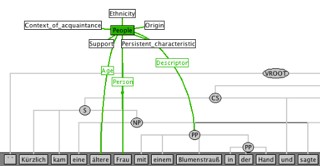
\includegraphics[scale=0.62]{images/frau1.png}
		\end{figure}
	}
	% \frame{
	% 	\begin{columns}[T]
	% 	    \begin{column}{.5\textwidth}
	% 		    \begin{block}{hello}
	% 		    \end{block}
	% 	    \end{column}
	% 	    \begin{column}{.5\textwidth}
	% 		    \begin{block}{Your image}
	% 		    
\includegraphics[width=.2\textwidth]{images/alpha.jpg}
	% 		    \end{block}
	% 	    \end{column}
	% 	\end{columns}
 %  }
	\frame{
		\frametitle{Motivation}
			\begin{itemize}[label=$\bullet$,itemsep=1.5ex]
				\item<1-> Rollen sind die letzten Bausteine, auf denen die semantische Information eines Satzes basiert
				\item<2-> Annotation von semantischen Rollen ist sehr hilfreich f\"ur alle \textbf{sprachverstehen}-bezogenen Aufgaben
			\end{itemize}
						\begin{columns}
							\onslide<3->{
							\begin{column}[c]{.4\textwidth}
								\textit{Opinion Mining}
				   			\end{column}
				   			}
			   				\onslide<4->{
			   				\begin{column}[c]{.4\textwidth}
								\textit{Watson (IBM)}
							\end{column}
							}
							\onslide<5->{
							\begin{column}[c]{.2\textwidth}
								
\includegraphics[scale=.1]{images/alpha.jpg}
						    \end{column}
						    }
						\end{columns}
				\begin{itemize}[label=$\bullet$,itemsep=1.5ex]
				\item<6-> Linguistische Forschung mit Bezug auf lexikalische Semantik
					\begin{itemize}[label=$-$,itemsep=1ex]
						\item<7-> Metapherntheorie: Ein Frame wird in Form eines anderen konzipiert
					\end{itemize}
			\end{itemize}
		%Anwendungsbeispiele 
		%Informationextraktion,...
		%Warum Rollen? theoretisches Beispiel
		%nicht aufschreiben, aber sagen - the linguists scarcity problem, zu viele daten zu wenige linguisten
	}

\section{\scshape Problemstellung}

	\frame{\frametitle{Gliederung} \tableofcontents[currentsection]}
	
	\frame{
		\frametitle{Problemstellung}
		\centering
		$\Longrightarrow$Automatische Bestimmung von Rollen:\\
		\vspace{1cm} 
		%\fbox{\parbox{\dimexpr \linewidth - 2\fboxrule - 2\fboxsep}{
		%\fbox{\parbox{\linewidth}{		
		\begin{quotation}
			\justifying
				\indent{\textit{Lassen sich semantische Rollen anhand von lexikalischen und 
				syntaktischen Informationen eines Satzes automatisch bestimmen?}}
		\end{quotation}
		%box rum blauer Rahmen
	}

	\frame{
		\frametitle{Corpus: Salsa 2.0}
		\begin{itemize}[label=$\bullet$,itemsep=1.5ex]
			\item<1-> Erstellt von der Universität Saarland \cite{rehbeinadding2012}
			\begin{itemize}[label=$-$,itemsep=1ex]
			  	% http://www.coli.uni-saarland.de/projects/salsa/corpus/doc/license.html
				\item frei für akademische Zwecke
			\end{itemize}
			% weiterentwicklung des SALSA 1.0
			\item<2-> Basiert auf dem TIGER-Korpus \cite{tiger}
			\begin{itemize}[label=$-$,itemsep=1ex]
				\item Treebank über Zeitungsartikel
				\item NEGRA Tag-Set
				\item
					viele morpho-syntaktische Informationen:\\ % Syntax: Phrasenkategorien, Syntaktische Funktionen, POS
					Pos-Tag, morphologische \& lemma-Informationen % Morphologie: Kasus-Genus usw... Lemma, POS
			\end{itemize}
			\item<3-> Frame-annortiertes Korpus
			\item<4-> Enthält: ~24.000 Sätze mit 648 Targets %target-word
			\item<5-> Targets: Nomen \& Verben
		\end{itemize}
	%	annotierung genau beschreiben (saetzengrenzen etc...)
	}	
	
	\frame{
		\frametitle{Corpus: Salsa 2.0}
		%Beispielbild von Salto: kurzer Satz mit edge-labels
		\begin{figure}
			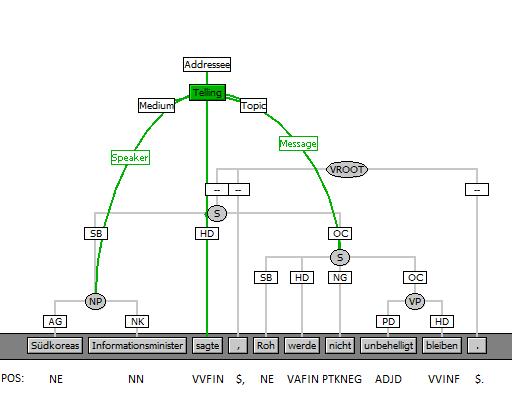
\includegraphics[scale=0.65]{images/s6544.png}
		\caption{semantisch annotierter Beispielsatz}
		\end{figure}
	}


\section{\scshape Umsetzung}
	
	\frame{\frametitle{Gliederung} \tableofcontents[currentsection]}

	\frame{
		\frametitle{Herangehensweise}
		\begin{itemize}[label=$\bullet$,itemsep=1.5ex]
			\item Analyse des Korpus bzgl. Struktur, Aufbau, Häufigkeitsverteilungen
			\item Ansatz von Jurafsky und Gildea\cite{gildea}
			\begin{itemize}[label=$-$,itemsep=1ex]
				\item Classifier: Naïve Bayes Classifier
				\item Angelehnte Features
			\end{itemize}
		\end{itemize}
	}
	\frame{
		\frametitle{Einschränkungen}
		\begin{figure}
		\centering
		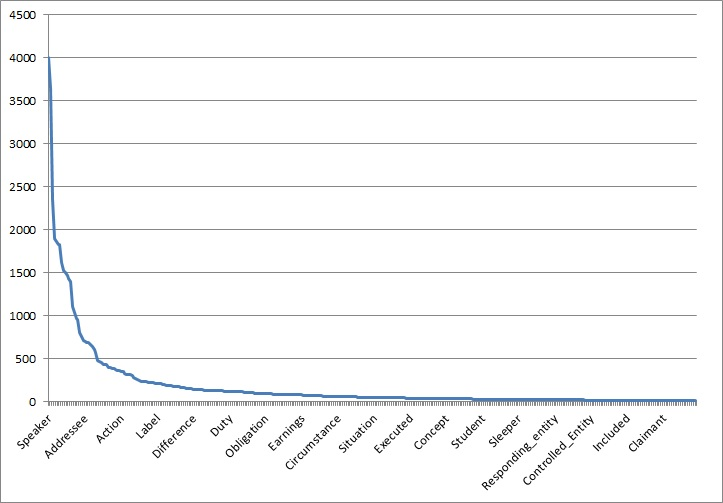
\includegraphics[scale=0.37]{images/roleFrequency.jpg}
		\caption{Verteilung der Rollen}
		\end{figure}
		\only<2->{$\Longrightarrow$Betrachtung der Top-10 Rollen}		
	}

	\frame{
		\frametitle{Einschränkungen (Forts.)}
		\begin{itemize}[label=$\bullet$,itemsep=1.5ex]
			\item<1-> Top-10 Rollen

			%\vspace{1cm}
			\item<2-> Keine Frames
			\begin{itemize}[label=$-$,itemsep=1ex]
				\item Disambiguierung zu komplex
			\end{itemize}

			%\vspace{1cm}
			\item<3->Target-Lemma muss bekannt sein
			\begin{itemize}[label=$-$,itemsep=1ex]
				\item Keine Abstraktion für ungesehene Targets
			\end{itemize}
		\end{itemize}
	}
	

	\frame{
		\frametitle{Prinzipieller Ablauf}
		\begin{itemize}
			\item<1->
			\begin{figure}
				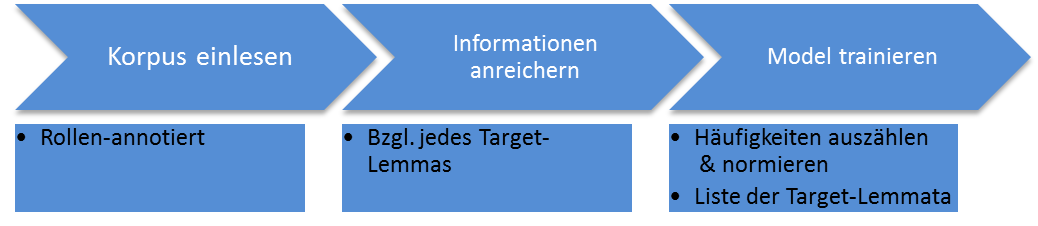
\includegraphics[scale=0.5]{images/ablaufLernen.png}
				\caption{Training}
			\end{figure}
			\item<2->
			\begin{figure}
				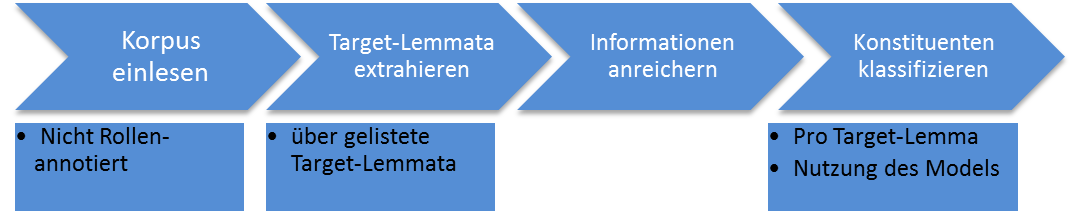
\includegraphics[scale=0.5]{images/ablaufAnnotate.png}
				\caption{Klassifikation}
			\end{figure}
		\end{itemize}
		%Keine Rolle
		%smoothing: 0.000001; threshold for frame: P(R1..Rk) > e^(-600)
	}

	\frame{
		\frametitle{Features}
		\begin{itemize}[label=$\bullet$,itemsep=1.5ex]
			\item<1-> Synt. Kategorie
			\begin{itemize}[label=$-$,itemsep=1ex]
				\item Nonterminal: phrasale Kategorie
				\item Terminal: POS-Tag
			\end{itemize}
		\end{itemize}

		\begin{figure}
			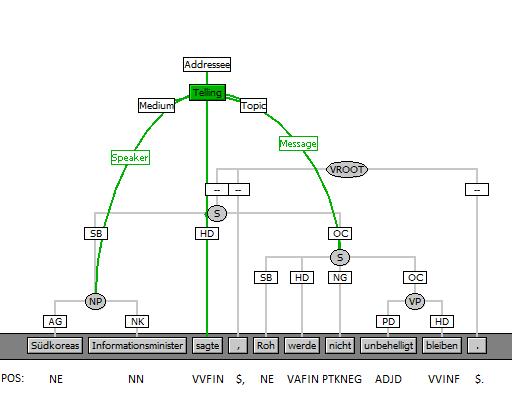
\includegraphics[scale=0.5]{images/s6544.png}
		\caption{semantisch annotierter Beispielsatz}
		\end{figure}
	}	
	\frame{
		\frametitle{Features (2)}
		\begin{itemize}[label=$\bullet$,itemsep=1.5ex]
			\item<1-> Pfad: über synt. Kategorien
			\begin{itemize}[label=$-$,itemsep=1ex]
				\item Zusammenfassen von Replikaten 
				\item Ignorieren von Konjunktionen
			\end{itemize}
		\end{itemize}
		\begin{figure}
			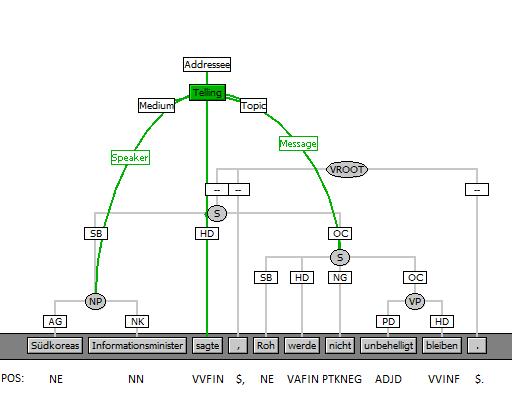
\includegraphics[scale=0.5]{images/s6544.png}
		\caption{semantisch annotierter Beispielsatz}
		\end{figure}
	}	
	\frame{
		\frametitle{Features (3)}
		\begin{itemize}[label=$\bullet$,itemsep=1.5ex]

			\item<1-> Position
			\begin{itemize}[label=$-$,itemsep=1ex]
				\item Position relativ zum Target
			\end{itemize}
		\end{itemize}
		\begin{figure}
			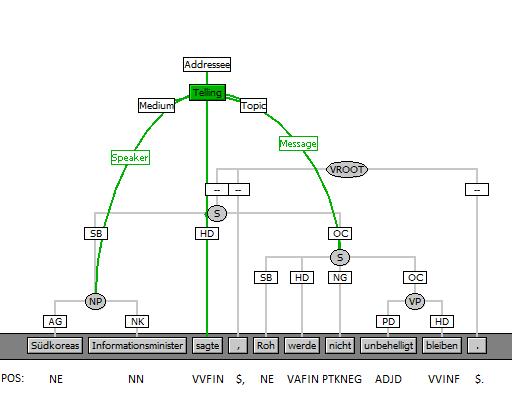
\includegraphics[scale=0.5]{images/s6544.png}
		\caption{semantisch annotierter Beispielsatz}
		\end{figure}
	}	
	\frame{
		\frametitle{Features (4)}
\begin{itemize}[label=$\bullet$,itemsep=1.5ex]
			\item<1-> Kopf-Lemma
			\begin{itemize}[label=$-$,itemsep=1ex]
				\item Syntaktisches Zentrum einer Phrase %TODO
				\item wird regelbasiert gesucht
				%terminal =  eigenes lemma als head
			\end{itemize}
		\end{itemize}
		\begin{figure}
			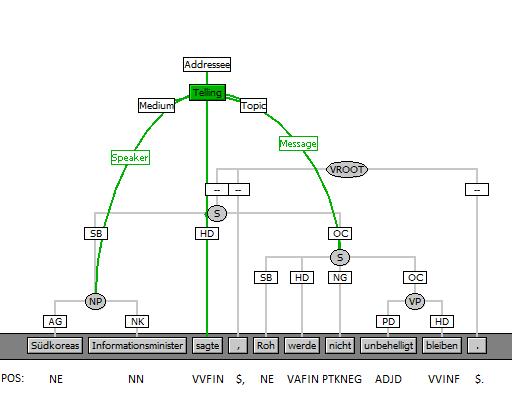
\includegraphics[scale=0.5]{images/s6544.png}
		\caption{semantisch annotierter Beispielsatz}
		\end{figure}
	}	
	\frame{
		\frametitle{Features (5)}
		\begin{itemize}[label=$\bullet$,itemsep=1.5ex]		
			\item<1-> Nachbar-Kopf-Lemma
			\begin{itemize}[label=$-$,itemsep=1ex]
				\item Kopf der einbettenden Konstituente
			\end{itemize}

			
		\end{itemize}
		\begin{figure}
			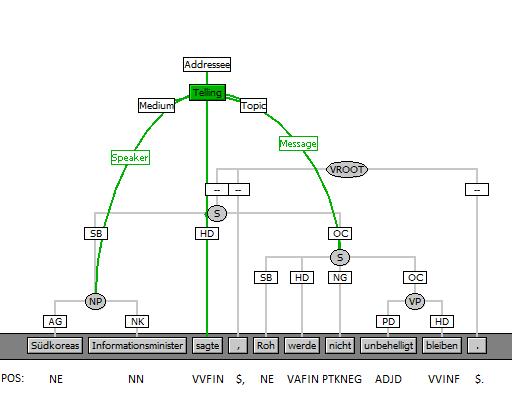
\includegraphics[scale=0.5]{images/s6544.png}
		\caption{semantisch annotierter Beispielsatz}
		\end{figure}
	}	
	\frame{
		\frametitle{Features (6)}
		\begin{itemize}[label=$\bullet$,itemsep=1.5ex]

			\item<1-> Kombination: Synt. Kat. \& Pfad
		\end{itemize}
		\begin{figure}
			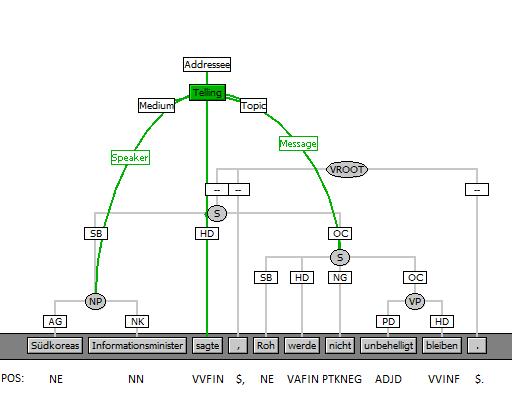
\includegraphics[scale=0.5]{images/s6544.png}
		\caption{semantisch annotierter Beispielsatz}
		\end{figure}
	}	

%	\frame{
% % Kommentar in der E-Mail an Leser: Features einzeln mit einem Bild kurz erklären statt KOmpakt + Beispiel danach
%		\frametitle{Features}
%		\begin{itemize}[label=$\bullet$,itemsep=1.5ex]
%			\item<1-> Synt. Kategorie
%			\begin{itemize}[label=$-$,itemsep=1ex]
%				\item Nonterminal: phrasale Kategorie
%				\item Terminal: POS-Tag
%			\end{itemize}
%			
%			%\vspace{1cm}
%			\item<2-> Pfad: über synt. Kategorien
%			\begin{itemize}[label=$-$,itemsep=1ex]
%				\item Zusammenfassen von Replikaten 
%				\item Ignorieren von Konjunktionen
%			\end{itemize}
%
%			%\vspace{1cm}
%			\item<3-> Position
%			\begin{itemize}[label=$-$,itemsep=1ex]
%				\item Position relativ zum Target
%			\end{itemize}
%		\end{itemize}
%	}
%
%	\frame{
%		\frametitle{Features (2)}
%		\begin{itemize}[label=$\bullet$,itemsep=1.5ex]
%			\item<1-> Kopf-Lemma
%			\begin{itemize}[label=$-$,itemsep=1ex]
%				\item Syntaktisches Zentrum einer Phrase %TODO
%				\item wird regelbasiert gesucht
%				%terminal =  eigenes lemma als head
%			\end{itemize}
%
%			%\vspace{1cm}			
%			\item<2-> Nachbar-Kopf-Lemma
%			\begin{itemize}[label=$-$,itemsep=1ex]
%				\item Kopf der einbettenden Konstituente
%			\end{itemize}
%
%			%\vspace{1cm}
%			\item<3-> Kombination: Synt. Kat. \& Pfad
%		\end{itemize}
%	}
%
%	\frame{
%		\frametitle{Features (3)}
%		\begin{figure}
%			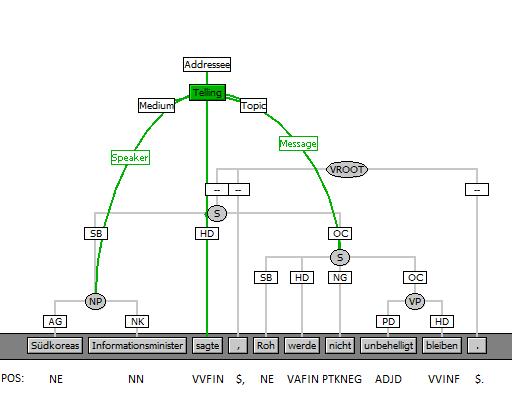
\includegraphics[scale=0.65]{images/s6544.png}
%		\caption{semantisch annotierter Beispielsatz}
%		\end{figure}
%	}	

	\frame{ % ZEILENABSTAND
		\frametitle{Probleme}
		\begin{itemize}[label=$\bullet$,itemsep=1.5ex]
			\item<1-> Deutsch: relativ freie Verschiebung von Konstituenten %Subjekt nicht auf die Vorfeldposition beschränkt....
			\item<2-> Kopf nicht überall definiert (NEGRA Tag-Set)
			%\item<3-> Querverbindung im Syntaxgraph % KOAN BAUM
		\end{itemize}
		\begin{itemize}[itemsep=1.5ex]
			\item<2-> \textcolor{white}{Target im Satz identifizieren}
			\begin{itemize}[itemsep=1ex]
				\item<2-> \textcolor{white}{Den Vortrag \textit{auf die lange Bank schieben.}}
				\item<2-> \textcolor{white}{Ich \textit{brach} den Ast \textit{ab.}}
			\end{itemize}			
		\end{itemize}
	}
	\frame{
		\frametitle{Probleme}
				\begin{figure}
					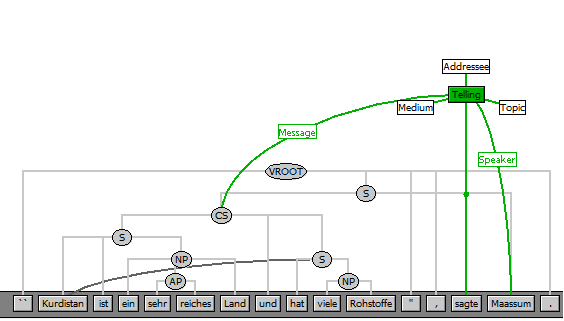
\includegraphics[scale=.7]{images/s2382.png}
					\caption{Querverbindung}
				\end{figure}
	}
	\frame{
		\frametitle{Probleme}
		\begin{itemize}[label=$\bullet$,itemsep=1.5ex]
			\item<1-> Deutsch: relativ freie Verschiebung von Konstituenten %Subjekt nicht auf die Vorfeldposition beschränkt....
			\item<1-> Kopf nicht überall definiert (NEGRA Tag-Set)
			\item<1-> Querverbindung im Syntaxgraph 
			% \begin{itemize}[label=$-$,itemsep=1ex]
				% \item<5-> Ich ging nach Haus' und aß Abendbrot. (Bild?)
			% \end{itemize}			
			\item<2-> Target im Satz identifizieren
			\begin{itemize}[label=$-$,itemsep=1ex]
				\item<3-> Den Vortrag \textit{auf die lange Bank schieben.}
				\item<4-> Ich \textit{brach} den Ast \textit{ab.}
			\end{itemize}			
		\end{itemize}
	}	


\section{\scshape Evaluation}
	\frame{\frametitle{Gliederung} \tableofcontents[currentsection]}

	\frame{
		\frametitle{Evaluation}
		\begin{itemize}[label=$\bullet$,itemsep=1.5ex]
			\item<1-> Target-Lemma muss vorhanden sein
			\begin{itemize}[label=$-$,itemsep=1ex]
				\item<1-> keines gefunden: Satz komplett ignoriert
			\end{itemize}
%da wir eine feste liste von target lemmata nutzen und nicht auf ungesehene targets abstrahieren koennen beruecksichtigen wird bei der evaluation nur 
%frame elements mit dem bezug auf ein (im Model) bekanntes target. counts erklaeren und ausgeben 
			\item<2-> Nutzung des F-Measure
			\begin{itemize}[label=$-$,itemsep=1ex]
				\item<2-> Sehr, sehr häufig: keine Rolle % accuracy dadurch unpassend
			\end{itemize}

			\item<3-> Precision
			\begin{itemize}[label=$-$,itemsep=1ex]
				\item<3-> P = $\dfrac{\#\text{(Korrekte Rolle klassifiziert)}}{\#\text{(Klassifiziert mit Rolle)}}$
			\end{itemize}				

			\item<3-> Recall
			\begin{itemize}[label=$-$,itemsep=1ex]
				\item<3-> R = $\dfrac{\#\text{(Korrekte Rolle klassifiziert)}}{\#\text{(Konstituenten mit Rolle)}}$
			\end{itemize}				
		\end{itemize}
	}

	\frame{
		\frametitle{Auswertung bezüglich dreier Kenngrößen}
		\begin{itemize}[itemsep=1.5ex] %TODO: should be enumerate
			\item<1->[1.] Konstituente wurde korrekte Rolle zugewiesen
			\begin{itemize}[label=$-$,itemsep=1ex]
				\item<1-> Exakte Übereinstimmung
			\end{itemize}
			\item<2->[2.] Konstituente wurde eine bel. Rolle zugewiesen
			\begin{itemize}[label=$-$,itemsep=1ex]
				\item<2-> Unabhängig von der Rolle
			\end{itemize}
			\item<3->[3.] Korrekte Rolle wurde im Satz gefunden
			\begin{itemize}[label=$-$,itemsep=1ex]
				\item<3-> Unabhängig von der Position im Satz
			\end{itemize}
		\end{itemize}
		% das letzte geht mehr auf die Rollenzählung ein, die ersten beiden sind für Konstituenten
	}

	\frame{
		\begin{figure}
			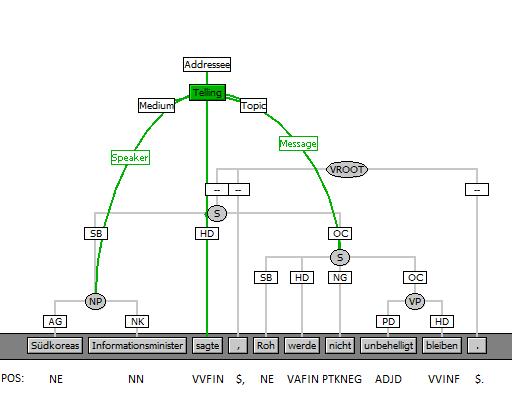
\includegraphics[scale=0.65]{images/s6544.png}
			\caption{semantisch annotierter Beispielsatz}
		\end{figure}%TODO Beispielsatz von Salto wieder nutzen, muss mind. 2 Rollen haben
	}


	\frame{
		\frametitle{Ergebnisse}
		\begin{itemize}[label=$\bullet$,itemsep=1.5ex]
		  \item Korpus: Top-10 Rollen
		  \begin{itemize}[itemsep=1ex]
			  \item $\sim$ 14000 Sätzen \& $\sim$ 22500 Konstituenten mit Rolle
		  \end{itemize}
		\end{itemize}

		\begin{figure}
			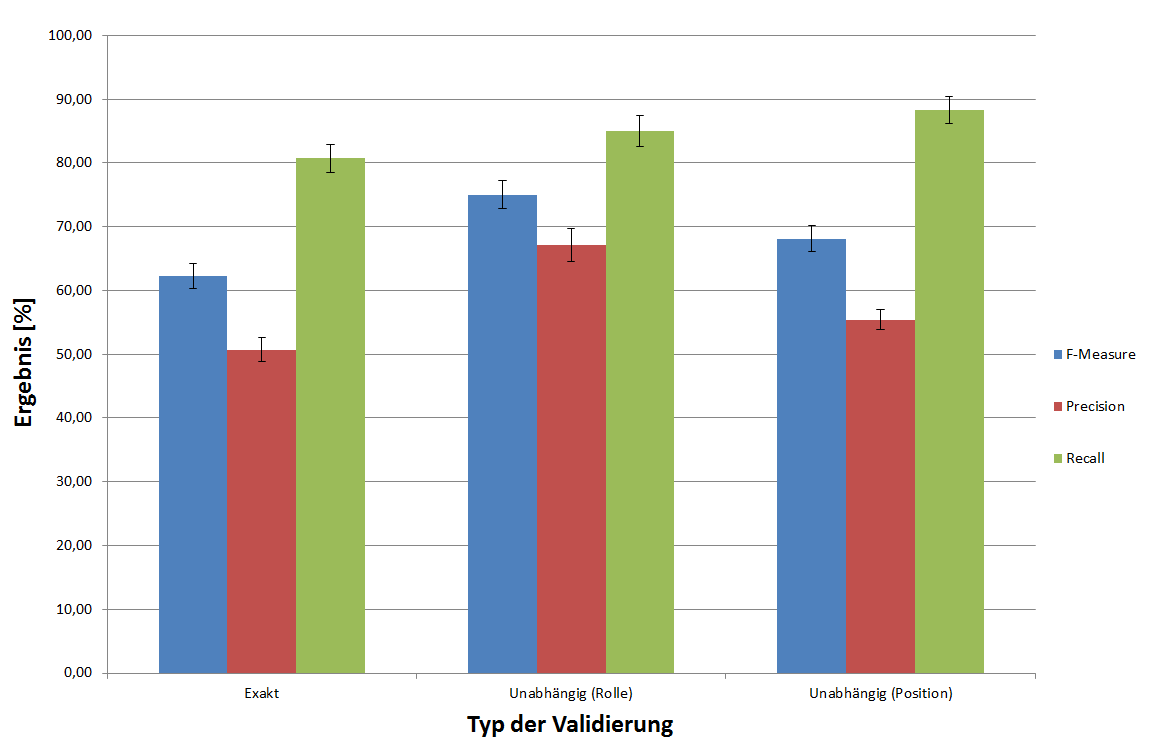
\includegraphics[width=0.8\textwidth]{images/ergebnisseKreuzvalidierung.png}
			\caption{5-fach Kreuzvalidierung [F1=0,62 $\vert$ P=0,51 $\vert$ R=0,81]}
		\end{figure}

		%\vspace{1cm}
% 		\begin{table}
% 			\small
% 			\caption{Ergebnisse einer 5-fach Kreuzvalidierung}
% 			\begin{tabular}{r|c|c|c}
% 			  	\toprule
% 			  	Typ						& \textbf{Precision} & \textbf{Recall} & \textbf{F-Measure} \\
% 			  	\midrule
% 				Exaktes Match 			&  0,51 $\pm$ 0,02 & 0,81 $\pm$ 0,02 & 0,62 $\pm$ 0,02 \\
% 				Unabhängig (Rolle)		&  0,67 $\pm$ 0,03 & 0,85 $\pm$ 0,02 & 0,75 $\pm$ 0,02 \\
% 				Unabhängig (Position)	&  0,55 $\pm$ 0,02 & 0,88 $\pm$ 0,02 & 0,68 $\pm$ 0,02 \\
% 				\bottomrule
% 			\end{tabular}
% 		\end{table}
% 
% 		\begin{flushright}
% 			\small
% 			\textit{Angabe: Ergebniswert (gerundet) $\pm$ Standardabweichung}
% 		\end{flushright}
	}

	\frame{
		\frametitle{Einordnung der Ergebnisse}
		\begin{itemize}[label=$\bullet$,itemsep=1.5ex]
			\item<1-> Erstes SRL-Projekt auf dem SALSA 2.0 Korpus
			%\vspace{1cm}
			\item<2-> SHALMANESER \cite{erk2006shalmaneser}
				% Universität Saarland
			\begin{itemize}[label=$-$,itemsep=1ex]
				\item<2-> Grundlage: SALSA 1.0 \cite{burchardt2006salsa} 
				\item<2-> Prec.: 0.761  $\vert$ Recall: 0.496  $\vert$ F-Measure: 0.600
				\item<2-> Vorgehen \& Evaluation unklar
			\end{itemize}

			%\vspace{1cm}
			\item<3-> Target-Lemma muss vorhanden sein
			\begin{itemize}[label=$-$,itemsep=1ex]
				\item<3-> 92\% der Konstituenten im Korpus ignoriert 
				%TODO  = (IDrefs overall - classified idrefs) / idrefs overall * 100
			\end{itemize}	
			\begin{itemize}
				\item<4-> $\Longrightarrow$ besserer Recall $\Longrightarrow$ besserer F-Measure
			\end{itemize}
			
		\end{itemize}
	}

	\frame{
		\frametitle{Einordnung der Ergebnisse (fort.)}
		
		\begin{figure}
			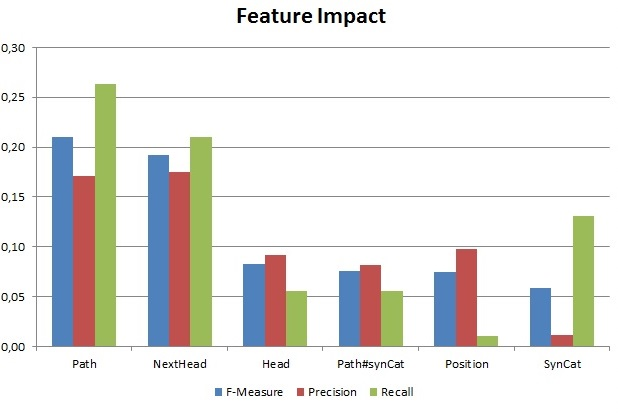
\includegraphics[scale=0.65]{images/featureImpact.jpg}
			\caption{Bedeutendste Features: Pfad \& Nachbar-Kopf}
		\end{figure}
		%\item Bedeutendste Features: Pfad \& Nachbar-Kopf
				% im Durchschnitt: 20% bzw. 15%
	}
	
	\frame{
		\frametitle{Mögliche Verbesserungen}
		\begin{itemize}[label=$\bullet$,itemsep=1.5ex]
			\item<1-> Vorverarbeitungsschritt: Dependenzgraph erzeugen
			\item<2-> Frames disambiguieren
			\item<3-> Semantische Abstraktion mit GermaNet
			\item<4-> Nutzung von Tree-Kernels
		\end{itemize}
		\vspace{0.5cm}
		\begin{itemize}	
			\item<5-> $\Longrightarrow$ mehr \& bessere Features!
		\end{itemize}
		
	}

	\frame{
		\centering
		\begin{Large} 
			Vielen Dank für die Aufmerksamkeit! \\
		\end{Large}
		\vspace{1cm}
		\begin{tikzpicture}[decoration=Koch curve type 2] 
			\draw[DeepSkyBlue4] decorate{ decorate{ decorate{ (0,0) -- (2,0) }}}; 
		\end{tikzpicture} \\
		\vspace{1cm}
		\begin{normalsize}
			Fragen?
		\end{normalsize}
	}


%%%% Referenzen
% \section*{\scshape Referenzen}
\scriptsize
\begin{frame}{Referenzen}
\tiny{\bibliographystyle{apalike} }
\bibliography{biblio}
\end{frame}

%%%%%

	\frame{
		\frametitle{Backup}
	}	

	\frame{
		% 2 Task: dependency parsing + semantic role labeling (zur Verfügung:
		% Head, Dependency-Graph, Syntaktische + Morph Informationen: Lemma, POS,
		% others) Tabelle: Nur Semantic Role Labeling Task
		\frametitle{Einordnung der Ergebnisse}
		\centering
        \begin{table}
		\adjustbox{max height=\dimexpr\textheight-5.5cm\relax,
          		   max width=\textwidth}{
		\begin{tabular}{cc|cccccccc}
		\toprule
		\textbf{Rank}   &    \textbf{System}   &    \textbf{Average}   &    \textbf{Catalan}   &    \textbf{Chinese}   &    \textbf{Czech}   &    \textbf{English}   &    \textbf{German} & \textbf{Japanese}   &    \textbf{Spanish} \\
		\midrule
		 1 &    Zhao   &    80.47   &    \textbf{80.32}   &    77.72   &    85.19   &    85.44   &    75.99   &    \textbf{78.15}   &    \textbf{80.46} \\
		 2 &    Nugues   &    80.31   &    80.01   &    \textbf{78.60}   &    \textbf{85.41}   &    \textbf{85.63}   &    \textbf{79.71}   &    76.3   &    76.52 \\
		 3 &    Meza-Ruiz   &    77.46   &    78   &    77.73   &    75.75   &    83.34   &    73.52   &    76   &    77.91 \\
		 4 &    Baoli Li   &    69.26   &    74.06   &    70.37   &    57.46   &    69.63   &    67.76   &    72.03   &    73.54 \\
		 5 &    Moreau   &    66.49   &    65.6   &    67.37   &    71.74   &    72.14   &    66.5   &    57.75   &    64.33\\
		 6 &    Täckström   &    61.27   &    57.11   &    63.41   &    71.05   &    67.64   &    53.42   &    54.74   &    61.51\\
		 7 &    Lin   &    57.18   &    61.7   &    70.33   &    60.43   &    65.66   &    59.51   &    23.78   &    58.87\\
		\bottomrule
		\end{tabular}
		}
		\caption{CoNLL-2009 Shared Task, SRL-only Task, Semantic Labeled F1 \cite{hajivc2009conll}}
		\end{table}
	}


%%%%%%%%%%%%%%%%%%%%%%%%%%%%%%%%%%%%%%%%%%%%




% \frame{
% \frametitle{What are semantic  roles?}
% \begin{itemize}
% 	\item<2->
% 			\begin{xlist}
% 			\ex
% 			\gll Peter gibt Karl Geld.\\
% 			\footnotesize
% 			\textcolor{blue}{\textit{SOURCE}}
% 			\footnotesize
% 			{}
% 			\footnotesize
% 			\textcolor{blue}{\textit{RECIPIENT} }
% 			\footnotesize
% 			\textcolor{blue}{\textit{THEMA}}
% 			\\
% 			%\vspace{1cm}
% 	\item<3->
			
% 			\gll Karl bekommt Geld von Peter.\\
% 			\footnotesize
% 			\textcolor{blue}{\textit{RECIPIENT}}
% 			\footnotesize
% 			{}
% 			\footnotesize
% 			\textcolor{blue}{\textit{THEMA}}
% 			\footnotesize
% 			\textcolor{blue}{\textit{SOURCE}}
% 			\\
% 			\end{xlist}

			
% \end{itemize}
% }



 \end{document}
